%==============================================================================
%  EILOR --- MANUAL DE LEVANTAMIENTO Y USO
%  Documento INDEPENDIENTE (autocontenido). Compila solo con pdfLaTeX.
%  Diseño y portada estilo "Faceta" (replica el formato de MACRO ACTIVIDAD.docx).
%
%  COMPILACIÓN:
%     pdflatex manual
%     pdflatex manual        (2ª pasada: índice y referencias)
%==============================================================================
\documentclass[12pt,a4paper,oneside]{report}

%--- Idioma y codificación --------------------------------------------------
\usepackage[utf8]{inputenc}
\usepackage[T1]{fontenc}
\usepackage[spanish,es-noshorthands,es-tabla]{babel}
\usepackage{lmodern}
\usepackage{helvet}                       % Helvetica: sustituto de Franklin Gothic
\renewcommand{\familydefault}{\sfdefault} % documento en sans, como el .docx
\usepackage{microtype}

%--- Geometría (A4, márgenes del documento original) ------------------------
\usepackage{geometry}
\geometry{a4paper,left=2.3cm,right=2.0cm,top=2.4cm,bottom=2.0cm,headheight=31pt,headsep=9pt}
\usepackage{setspace}
\onehalfspacing
\usepackage{parskip}

%--- Gráficos, color, tablas ------------------------------------------------
\usepackage{graphicx}
\usepackage{xcolor}
\usepackage{float}
\usepackage{booktabs}
\usepackage{tabularx}
\usepackage{array}
\usepackage{enumitem}
\usepackage{amssymb}

%--- Diagramas y portada ----------------------------------------------------
\usepackage{tikz}
\usetikzlibrary{shapes.geometric,arrows.meta,positioning,calc}

%--- Paleta "Faceta" (tomada del tema del documento MACRO ACTIVIDAD) ---------
\definecolor{facetred}{HTML}{A4063E}   % accent1  (carmesí, color principal)
\definecolor{facetgreen}{HTML}{93C842} % accent2  (verde)
\definecolor{facetteal}{HTML}{1D7D74}  % accent3  (teal)
\definecolor{facetnavy}{HTML}{282660}  % dk2      (azul marino)
\definecolor{facetgrey}{HTML}{E6E7E8}  % lt2      (gris claro)
\definecolor{facetdark}{HTML}{161718}  % dk1
% Colores para los diagramas y enlaces (reapuntados a la paleta Faceta)
\colorlet{eilorcyan}{facetteal}
\colorlet{eiloremerald}{facetgreen}
\colorlet{eilordark}{facetnavy}
% Fondos de código
\definecolor{codebg}{RGB}{248,249,250}
\definecolor{codecomment}{RGB}{106,115,125}
\definecolor{codestring}{RGB}{3,71,120}
\definecolor{codekw}{HTML}{A4063E}
\definecolor{codendk}{HTML}{1D7D74}
% Fondos de cajas de aviso/nota
\definecolor{notabg}{HTML}{E4F1EF}
\definecolor{avisobg}{HTML}{F8E6EC}

%--- Títulos de capítulo y sección (estilo Faceta) --------------------------
\usepackage{titlesec}
\titleformat{\chapter}[hang]
  {\sffamily}
  {\colorbox{facetred}{\makebox[1.5cm][c]{\rule[-0.35cm]{0pt}{1.25cm}\color{white}\fontsize{34}{34}\selectfont\bfseries\thechapter}}}
  {14pt}
  {\color{facetnavy}\Huge\bfseries}
  [\vspace{4pt}{\color{facetgreen}\titlerule[2.5pt]}]
\titlespacing*{\chapter}{0pt}{6pt}{20pt}
\titleformat{\section}{\sffamily\Large\bfseries\color{facetred}}{\thesection}{0.6em}{}
\titleformat{\subsection}{\sffamily\large\bfseries\color{facetteal}}{\thesubsection}{0.6em}{}
\titleformat{\subsubsection}{\sffamily\normalsize\bfseries\color{facetnavy}}{\thesubsubsection}{0.6em}{}

%--- Encabezados y pies (estilo Faceta: pestaña carmesí con el nº de página) -
\usepackage{fancyhdr}
\newcommand{\pagetab}{\colorbox{facetred}{\makebox[1.05cm][c]{\rule[-0.18cm]{0pt}{0.62cm}\color{white}\bfseries\thepage}}}
\renewcommand{\chaptermark}[1]{\markboth{#1}{}}
\pagestyle{fancy}
\fancyhf{}
\fancyhead[L]{\footnotesize\color{facetnavy}\textsc{EILOR --- Manual de levantamiento y uso}}
\fancyhead[R]{\pagetab}
\renewcommand{\headrule}{\hbox to\headwidth{\color{facetred}\leaders\hrule height 1.2pt\hfill}}
\fancyfoot[L]{\footnotesize\color{gray}Sistemas de Información y Ciberseguridad}
\fancyfoot[R]{\footnotesize\color{gray}\thepage}
\renewcommand{\footrulewidth}{0.4pt}
\fancypagestyle{plain}{%
  \fancyhf{}%
  \fancyhead[R]{\pagetab}%
  \renewcommand{\headrule}{\hbox to\headwidth{\color{facetred}\leaders\hrule height 1.2pt\hfill}}%
  \fancyfoot[L]{\footnotesize\color{gray}Sistemas de Información y Ciberseguridad}%
  \fancyfoot[R]{\footnotesize\color{gray}\thepage}%
  \renewcommand{\footrulewidth}{0.4pt}}

%--- Listados de código -----------------------------------------------------
\usepackage{listings}
\lstdefinelanguage{JavaScript}{
  keywords={const,let,var,function,return,if,else,for,while,do,new,require,module,exports,async,await,try,catch,finally,typeof,class,this,break,switch,case,default,true,false,null,undefined,in,of,throw,delete},
  keywordstyle=\color{codekw}\bfseries,
  ndkeywords={console,JSON,Date,Math,Array,Map,Set,Object,Promise,express,app,res,req,ws,wss,process,setInterval,setTimeout,fetch,document},
  ndkeywordstyle=\color{codendk},
  sensitive=true,comment=[l]{//},morecomment=[s]{/*}{*/},
  morestring=[b]",morestring=[b]',morestring=[b]`
}
\lstset{
  backgroundcolor=\color{codebg},
  basicstyle=\ttfamily\footnotesize,
  commentstyle=\color{codecomment}\itshape,
  stringstyle=\color{codestring},
  keywordstyle=\color{codekw}\bfseries,
  numbers=left,numberstyle=\tiny\color{gray},numbersep=8pt,
  breaklines=true,breakatwhitespace=false,
  frame=single,rulecolor=\color{facetgrey},
  showstringspaces=false,tabsize=2,captionpos=b,extendedchars=true,
  literate=%
    {á}{{\'a}}1 {é}{{\'e}}1 {í}{{\'i}}1 {ó}{{\'o}}1 {ú}{{\'u}}1
    {ñ}{{\~n}}1 {Ñ}{{\~N}}1 {ü}{{\"u}}1 {Ü}{{\"U}}1
    {¿}{{?`}}1 {¡}{{!`}}1 {°}{{\textdegree}}1
}
\lstdefinestyle{js}{language=JavaScript}
\lstdefinestyle{cpp}{language=C++}
\lstdefinestyle{bash}{language=bash,keywordstyle=\color{facetgreen}\bfseries}

%--- Enlaces ----------------------------------------------------------------
\usepackage[hidelinks]{hyperref}
\hypersetup{
  colorlinks=true,linkcolor=facetnavy,urlcolor=facetteal,citecolor=facetteal,
  pdftitle={EILOR --- Manual de levantamiento y uso},
  pdfauthor={Proyecto EILOR}
}

%--- Comandos de ayuda ------------------------------------------------------
\newcommand{\code}[1]{\texttt{\small #1}}
\newcommand{\plataformaurl}{\url{https://esp.orellanadigitalco.trade/}}
\newcommand{\repourl}{\url{https://github.com/ptandazoz9827/evil-esp32}}
% Datos editables de la carátula. Sustituya estos valores cuando se confirmen.
\newcommand{\nombreestudiante}{Pablo Alejandro Tandazo Zarango}
\newcommand{\direccionestudiante}{Dirección}
\newcommand{\ciudadestudiante}{Ciudad, provincia y código postal}
\newcommand{\telefonoestudiante}{Teléfono}
\newcommand{\correoestudiante}{Correo electrónico}

% Inserta una captura/fotografía real (archivo en figuras/, sin extensión)
\newcommand{\captura}[3][0.85]{%
  \begin{figure}[H]\centering
  \setlength{\fboxsep}{0pt}\setlength{\fboxrule}{0.6pt}%
  \fcolorbox{facetgrey}{white}{\includegraphics[width=#1\linewidth]{figuras/#2}}%
  \caption{#3}\end{figure}}

% Placeholder para fotografías aún no disponibles
\newcommand{\capturapend}[2][0.7]{%
  \begin{figure}[H]\centering
  \fbox{\begin{minipage}[c][3.6cm][c]{#1\linewidth}\centering
  \textcolor{gray}{\ttfamily [ FOTOGRAFÍA PENDIENTE ]}\\[4pt]
  \small\textcolor{gray}{#2}\end{minipage}}
  \caption{#2}\end{figure}}

% Cajas de aviso y nota (colores Faceta)
\newcommand{\cajanota}[2]{%
  \par\smallskip\noindent
  \fcolorbox{facetteal}{notabg}{\parbox{\dimexpr\linewidth-2\fboxsep-2\fboxrule}{%
  \textbf{\textcolor{facetteal}{\textbullet\ Nota --- #1}}\par\smallskip #2}}\par\smallskip}
\newcommand{\cajaaviso}[2]{%
  \par\smallskip\noindent
  \fcolorbox{facetred}{avisobg}{\parbox{\dimexpr\linewidth-2\fboxsep-2\fboxrule}{%
  \textbf{\textcolor{facetred}{$\triangle$\ Importante --- #1}}\par\smallskip #2}}\par\smallskip}

%============================================================================
\begin{document}

%--------------------------- PORTADA (estilo Faceta) ------------------------
\hypersetup{pageanchor=false}
\begin{titlepage}
\thispagestyle{empty}
\begin{tikzpicture}[remember picture,overlay]
  \coordinate (NW) at (current page.north west);
  % Fotografía de fondo a sangre completa
  \node[anchor=north west,inner sep=0] at (NW)
    {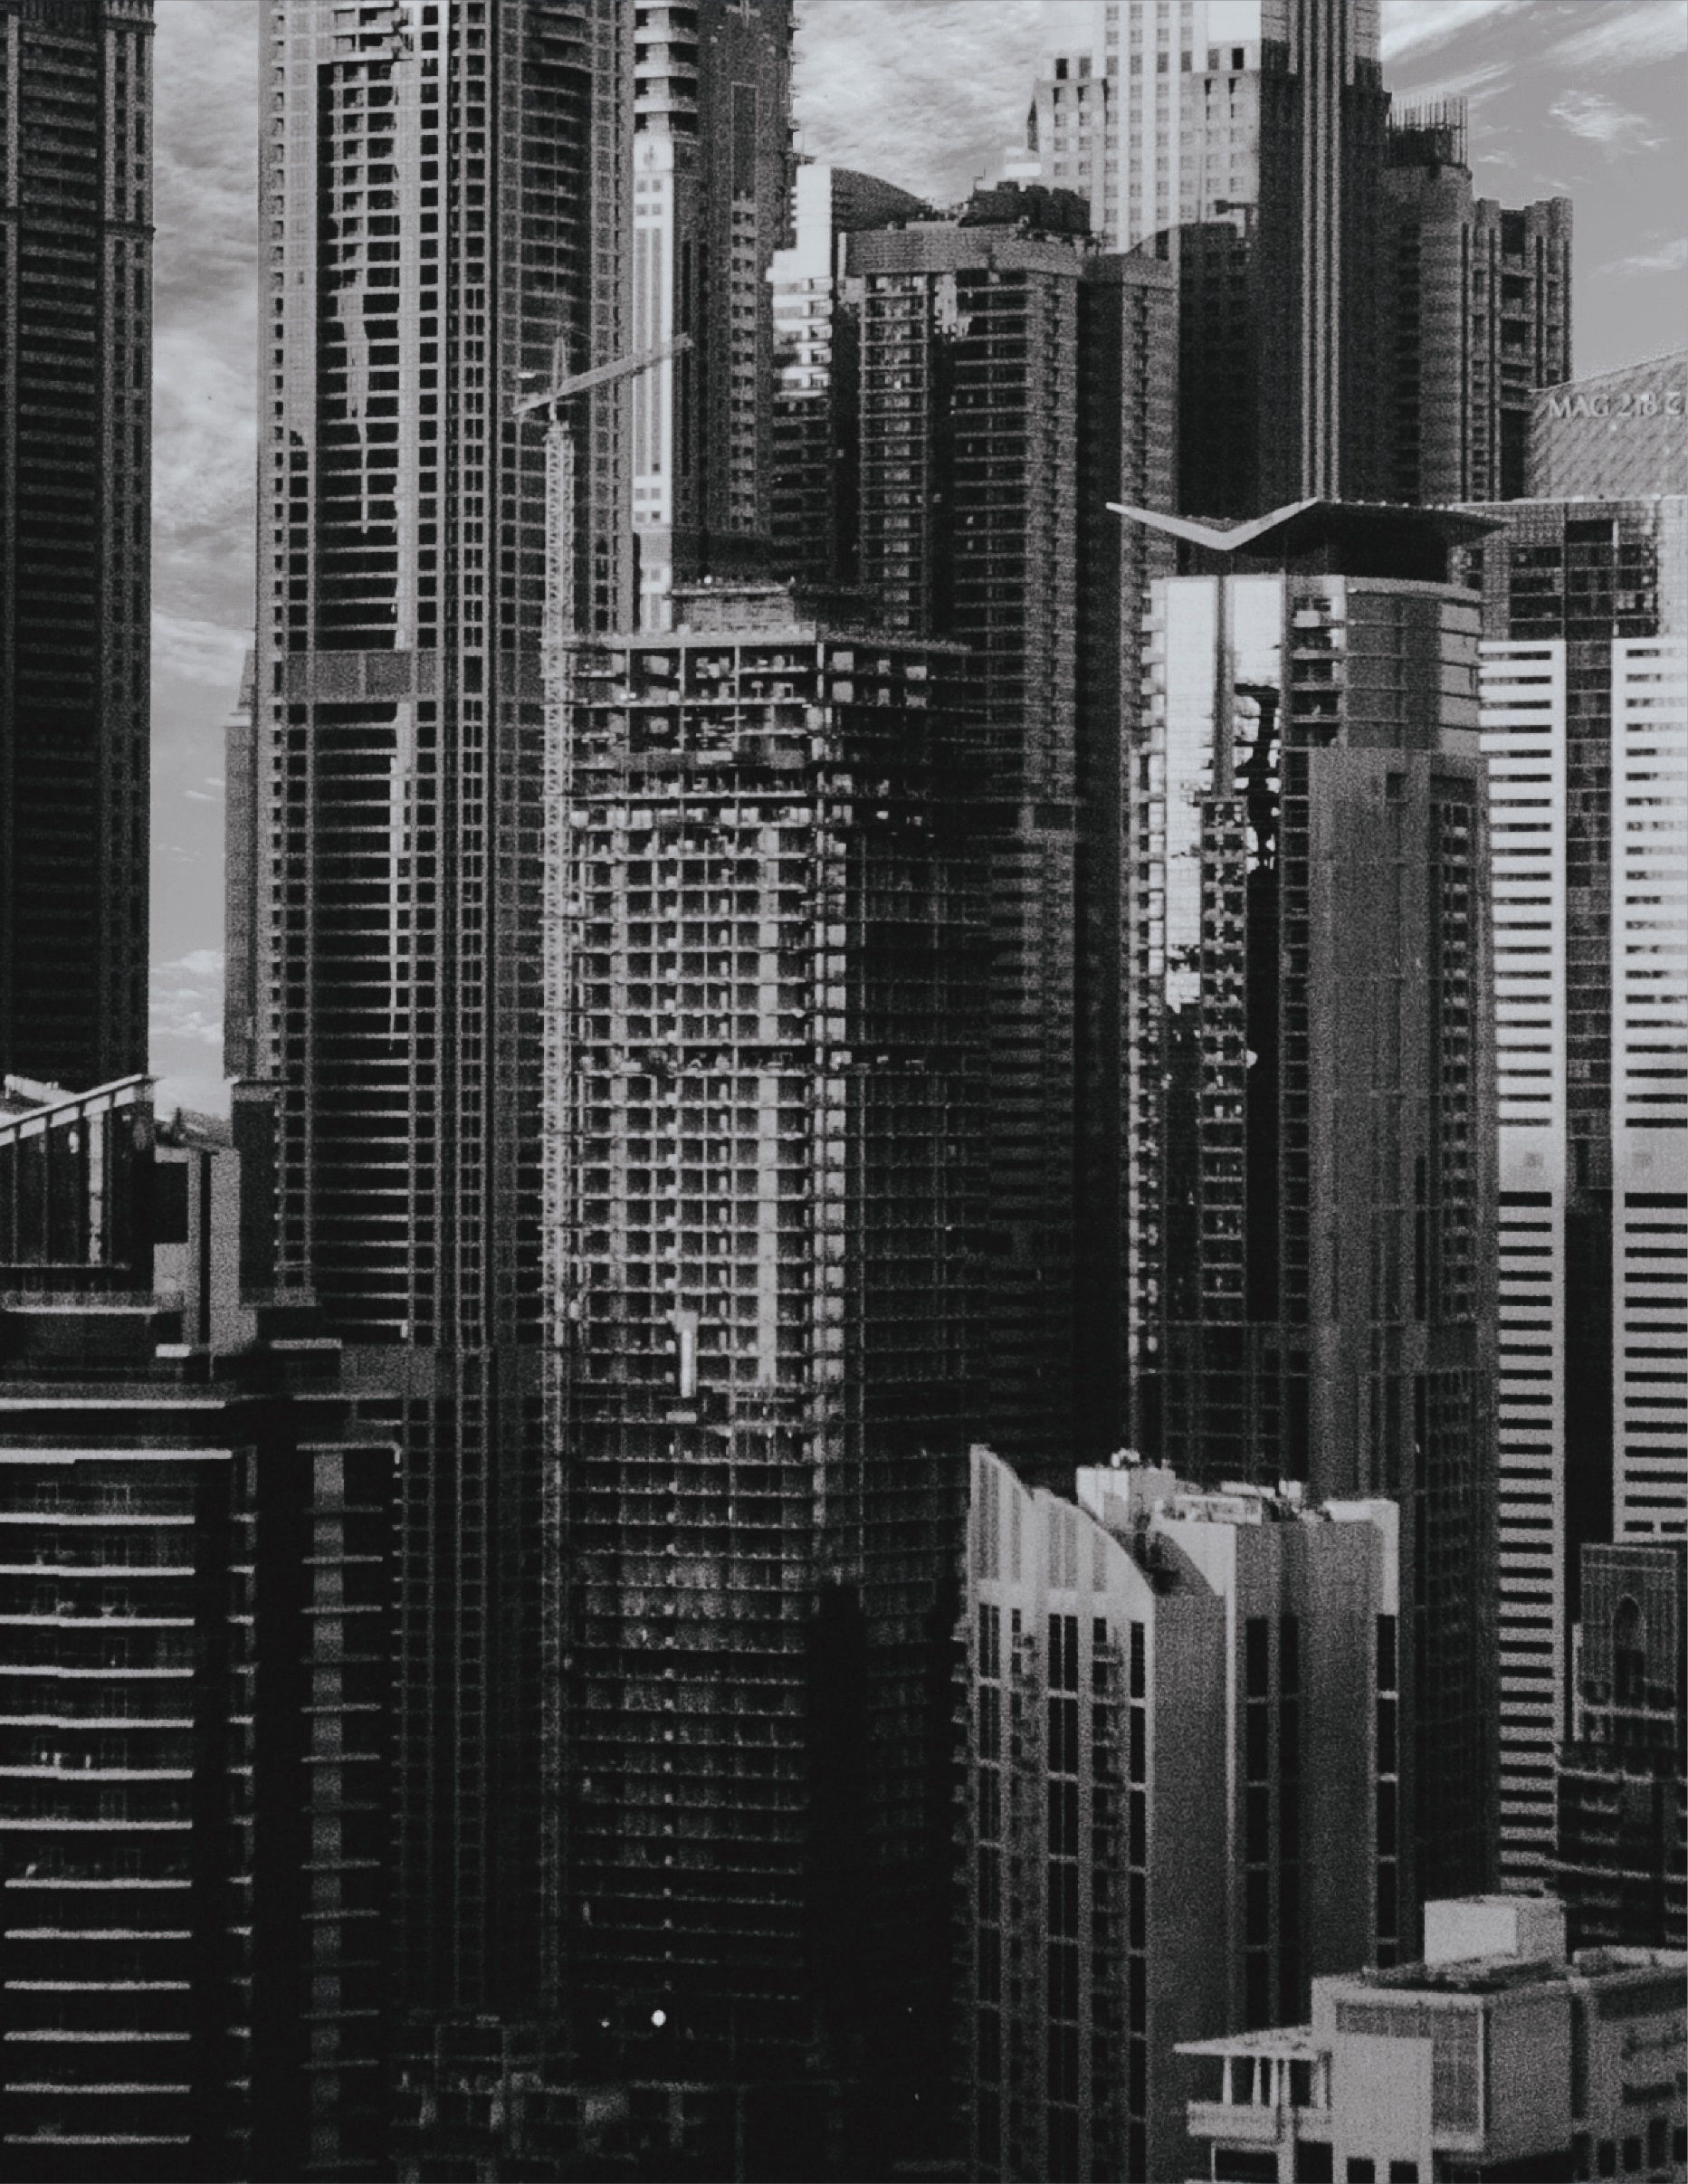
\includegraphics[width=\paperwidth,height=\paperheight]{figuras/portada-ciudad}};
  % Barra vertical verde (acento izquierdo)
  \fill[facetgreen] ([yshift=-18mm]NW) rectangle ([xshift=9mm,yshift=-95mm]NW);
  % Etiqueta superior
  \node[anchor=north west,text=white,align=left,font=\sffamily\bfseries\large]
    at ([xshift=16mm,yshift=-24mm]NW) {MANUAL TÉCNICO};
  \node[anchor=north west,text=white,align=left,font=\sffamily\small]
    at ([xshift=16mm,yshift=-33mm]NW) {Proyecto tecnológico en Sistemas de Información y Ciberseguridad};
  % Bloque carmesí con el título
  \fill[facetred,opacity=0.95] ([yshift=-150mm]NW) rectangle ([xshift=\paperwidth,yshift=-214mm]NW);
  \node[anchor=west,text=white,align=left,text width=175mm,font=\sffamily]
    at ([xshift=17mm,yshift=-182mm]NW)
    {{\fontsize{15}{17}\selectfont EILOR}\\[4pt]
     {\fontsize{34}{38}\selectfont\bfseries Manual de levantamiento y uso}\\[6pt]
     {\fontsize{12}{14}\selectfont\itshape Puesta en marcha de cada componente, operación y mantenimiento}};
  % Banda azul marino con subtítulo
  \fill[facetnavy] ([yshift=-214mm]NW) rectangle ([xshift=\paperwidth,yshift=-241mm]NW);
  \node[anchor=west,text=white,align=left,text width=175mm,font=\sffamily\bfseries]
    at ([xshift=17mm,yshift=-227.5mm]NW)
    {DESARROLLO DE PROYECTO TECNOLÓGICO EN SISTEMAS DE INFORMACIÓN Y CIBERSEGURIDAD};
  % Bloque inferior de datos (autor / contacto) sobre banda gris
  \fill[white,opacity=0.92] ([yshift=-241mm]NW) rectangle ([xshift=\paperwidth,yshift=-297mm]NW);
  \node[anchor=north west,text=facetdark,align=left,font=\sffamily,text width=120mm]
    at ([xshift=17mm,yshift=-247mm]NW)
    {\textbf{\color{facetred}\nombreestudiante}\\[2pt]
     \direccionestudiante\\ \ciudadestudiante\\
     \telefonoestudiante\\ \correoestudiante};
  % Logo institucional (abajo a la derecha)
  \node[anchor=south east,inner sep=0] at ([xshift=\paperwidth-16mm,yshift=-289mm]NW)
    {
\includegraphics[width=52mm]{figuras/logo-sic}};
  % Fecha
  \node[anchor=south west,text=facetnavy,font=\sffamily\small\bfseries]
    at ([xshift=17mm,yshift=-291mm]NW) {\today};
\end{tikzpicture}
\end{titlepage}

%--------------------------- ÍNDICE -----------------------------------------
\hypersetup{pageanchor=true}
\pagenumbering{roman}
\renewcommand{\contentsname}{\color{facetnavy}Contenido}
\tableofcontents
\clearpage
\pagenumbering{arabic}

%============================================================================
\chapter{Introducción y alcance del manual}
\label{cap:intro}

Este manual describe, paso a paso, cómo \textbf{levantar} (poner en marcha) cada uno
de los componentes que integran el sistema EILOR y cómo \textbf{operarlo} en el día
a día. Está pensado como documento autónomo: puede seguirse sin necesidad de
consultar el informe de tesis, aunque lo complementa.

El sistema se compone de cinco piezas que se levantan en orden:

\begin{enumerate}[leftmargin=1.9em]
  \item \textbf{Hardware} --- placa ESP32 con pantalla OLED, pulsador y alimentación.
  \item \textbf{Firmware} --- programa cargado en el ESP32 (cuatro modos de operación).
  \item \textbf{Servidor Node.js} --- recibe las mediciones, las persiste y sirve el dashboard.
  \item \textbf{Cloudflare Tunnel} --- publica el servidor en Internet con cifrado TLS, sin abrir puertos.
  \item \textbf{Dashboard web} --- interfaz de control y visualización en tiempo real.
\end{enumerate}

\section{Diagrama general del sistema}
La Figura~\ref{fig:sistema} resume cómo se relacionan los componentes: el ESP32
mide el entorno de 2.4~GHz y envía los datos por WebSocket seguro (WSS) al servidor;
los navegadores consumen el dashboard por HTTPS. Cloudflare termina el TLS en su
borde y reenvía el tráfico por un túnel saliente hasta el servidor local.

\begin{figure}[H]
\centering
\begin{tikzpicture}[
  font=\sffamily\small,
  n/.style={rectangle,rounded corners=3pt,draw,thick,align=center,minimum height=1.0cm,minimum width=2.5cm},
  arr/.style={-{Latex[length=2.4mm]},thick},
  lbl/.style={font=\sffamily\scriptsize\itshape,align=center}
]
\node[n,fill=facetteal!12] (esp) {ESP32\\+ OLED};
\node[n,fill=gray!8,below=0.8cm of esp] (web) {Navegador};
\node[n,fill=orange!14,right=2.4cm of esp,yshift=-0.7cm,minimum height=1.8cm] (edge) {Cloudflare\\Edge\\(TLS 443)};
\node[n,fill=facetgreen!18,right=2.2cm of edge] (cfd) {cloudflared\\(túnel)};
\node[n,fill=facetnavy!12,right=2.0cm of cfd] (srv) {Node.js\\:3002 (PM2)};
\draw[arr] (esp) -- node[lbl,above]{WSS} (edge);
\draw[arr] (web) -- node[lbl,below]{HTTPS} (edge);
\draw[{Latex[length=2.4mm]}-{Latex[length=2.4mm]},thick] (edge) -- node[lbl,above]{túnel\\cifrado} (cfd);
\draw[arr] (cfd) -- node[lbl,above]{HTTP\\local} (srv);
\end{tikzpicture}
\caption{Relación entre los componentes y el flujo de datos de extremo a extremo.}
\label{fig:sistema}
\end{figure}

\section{Requisitos previos}
\begin{table}[H]
\centering
\caption{Requisitos de hardware y software}
\footnotesize
\begin{tabularx}{\linewidth}{@{}l X@{}}
\toprule
\textbf{\color{facetnavy}Elemento} & \textbf{\color{facetnavy}Detalle} \\
\midrule
Placa & ESP32 DevKit (WROOM-32) \\
Pantalla & OLED SSD1306 0.96" I\textsuperscript{2}C (dirección 0x3C) \\
Entrada & Pulsador momentáneo (GPIO15, \code{INPUT\_PULLUP}) \\
Alimentación & Fuente USB 5~V capaz de entregar $\ge$500~mA \\
PC de desarrollo & Arduino IDE o PlatformIO, Node.js 18+ y \code{npm} \\
Cuenta & Cloudflare con un dominio propio (para el túnel) \\
Navegador & Cualquier navegador moderno para el dashboard \\
\bottomrule
\end{tabularx}
\end{table}

\cajaaviso{Uso responsable y legal}{El modo SoftAP con portal cautivo solo debe
emplearse en redes propias o expresamente autorizadas, con un SSID identificable y
con consentimiento informado de quienes se registran. No debe usarse para suplantar
redes de terceros ni para capturar datos sin autorización.}

%============================================================================
\chapter{Montaje del hardware ESP32}
\label{cap:hardware}

El primer componente físico a levantar es la placa ESP32 con su pantalla OLED y el
pulsador. La Figura~\ref{fig:electronico} muestra el diagrama de conexiones.

\captura[0.92]{diagrama-electronico-eilor}{Diagrama electrónico: ESP32, pantalla OLED por I\textsuperscript{2}C y pulsador.}
\label{fig:electronico}

\section{Conexionado (pinout)}
Realice el cableado \textbf{con la placa desconectada de toda fuente de energía}.
La Tabla~\ref{tab:pinout} detalla cada conexión.

\begin{table}[H]
\centering
\caption{Asignación de pines del ESP32}
\label{tab:pinout}
\footnotesize
\begin{tabularx}{\linewidth}{@{}l l l X@{}}
\toprule
\textbf{\color{facetnavy}Pin ESP32} & \textbf{\color{facetnavy}Señal} & \textbf{\color{facetnavy}Componente} & \textbf{\color{facetnavy}Notas} \\
\midrule
3V3 & Alimentación & OLED VCC & Lógica y alimentación a 3.3~V \\
GND & Común & OLED / Pulsador & Tierra compartida \\
GPIO21 & SDA (I\textsuperscript{2}C) & OLED & Datos del bus \\
GPIO22 & SCL (I\textsuperscript{2}C) & OLED & Reloj del bus \\
GPIO15 & Entrada digital & Pulsador & \code{INPUT\_PULLUP}; activo en bajo \\
\bottomrule
\end{tabularx}
\end{table}

\begin{enumerate}[leftmargin=1.9em]
  \item Conecte \textbf{OLED VCC} a \textbf{3V3} y \textbf{OLED GND} a \textbf{GND}.
  \item Conecte \textbf{SDA} de la OLED a \textbf{GPIO21} y \textbf{SCL} a \textbf{GPIO22}.
  \item Conecte una pata del \textbf{pulsador} a \textbf{GPIO15} y la otra a \textbf{GND}
        (no requiere resistencia externa: se usa la \emph{pull-up} interna).
  \item Revise que no haya cortos entre 3V3 y GND antes de energizar.
\end{enumerate}

\cajanota{Sobre la alimentación}{Use \emph{una sola} fuente a la vez. Para la primera
puesta en marcha, alimente por el cable USB del computador. Para operación autónoma,
use un portapilas con \textbf{salida USB regulada}; las pilas AA no se conectan
directamente a 3V3 ni a 5V.}

\section{Montaje físico del prototipo}
La Figura~\ref{fig:montaje} muestra el prototipo armado sobre \emph{protoboard}: la
placa ESP32, la pantalla OLED y el cableado I\textsuperscript{2}C, junto al monitor
serie que confirma la conexión.

\captura[0.9]{foto-montaje-monitor-serie}{Montaje físico del prototipo (ESP32 + OLED) y monitor serie durante la puesta en marcha.}
\label{fig:montaje}

\section{Carcasa y ubicación}
Si utiliza carcasa, siga la propuesta conceptual de la Figura~\ref{fig:carcasa}:
deje libre la zona frente a la antena y verifique que el pulsador pueda accionarse
sin abrir el equipo. Mantenga la placa alejada de superficies metálicas para no
degradar la medición de RF.

\captura[0.72]{carcasa-eilor-conceptual}{Propuesta conceptual de carcasa con acceso a USB, pulsador y zona libre frente a la antena.}
\label{fig:carcasa}

%============================================================================
\chapter{Levantamiento del firmware}
\label{cap:firmware}

El firmware es el programa que gobierna el ESP32. Se compila y carga desde
\textbf{Arduino IDE} o \textbf{PlatformIO}.

\section{Librerías requeridas}
Instale, desde el gestor de librerías, las siguientes dependencias:
\begin{itemize}[leftmargin=1.5em]
  \item \code{WebSockets} (Markus Sattler) --- cliente WebSocket/WSS.
  \item \code{Adafruit\_SSD1306} y \code{Adafruit\_GFX} --- control de la pantalla OLED.
  \item \code{ezButton} --- lectura del pulsador con antirrebote.
\end{itemize}

\section{Preparación de la carpeta}
Coloque el archivo \code{eilor\_esp32.ino} en una carpeta con \emph{su mismo nombre}
(\code{eilor\_esp32/}).

\section{Parámetros a configurar antes de compilar}
Edite en el firmware, como mínimo, los siguientes valores:

\begin{table}[H]
\centering
\caption{Parámetros de configuración del firmware}
\label{tab:fwconf}
\footnotesize
\begin{tabularx}{\linewidth}{@{}l X@{}}
\toprule
\textbf{\color{facetnavy}Parámetro} & \textbf{\color{facetnavy}Función} \\
\midrule
\code{WIFI\_SSID} / \code{WIFI\_PASS} & Credenciales de la red Wi-Fi de estación \\
\code{WS\_SERVER\_HOST} & Hostname público del servidor (p.\,ej. \code{esp.tu-dominio.com}) \\
\code{DEVICE\_TOKEN} & (Opcional) token que debe coincidir con el del servidor \\
\code{PORTAL\_TITULO} & (Opcional) título mostrado en el portal cautivo \\
\bottomrule
\end{tabularx}
\end{table}

\cajanota{Conexión segura}{El firmware se conecta con TLS mediante\\
\code{webSocket.beginSSL(WS\_SERVER\_HOST, 443, "/")}, coherente con la terminación
TLS que realiza Cloudflare en su borde (Capítulo~\ref{cap:cloudflare}).}

\section{Compilación y carga}
\begin{enumerate}[leftmargin=1.9em]
  \item Seleccione la placa \emph{ESP32 Dev Module} y el puerto serie correcto.
  \item Compile y cargue el \emph{sketch}.
  \item Abra el \textbf{monitor serie a 115200 baudios}.
\end{enumerate}

\section{Verificación por monitor serie}
Compruebe, \textbf{en este orden}, los mensajes de arranque: inicialización de la
OLED (0x3C), asociación Wi-Fi, conexión TLS (WSS) y mensajes de cambio de modo. La
Figura~\ref{fig:serie} muestra el monitor serie confirmando la conexión al servidor
y el envío de análisis de espectro.

\captura[0.78]{foto-oled-wifi-serie}{Monitor serie: asociación Wi-Fi, conexión WSS al servidor y análisis de espectro enviados.}
\label{fig:serie}

\cajaaviso{Si la pantalla no inicia}{Antes de volver a grabar, compruebe VCC, GND,
SDA, SCL y la dirección I\textsuperscript{2}C (0x3C). Consulte también la resolución
de problemas del Capítulo~\ref{cap:problemas}.}

%============================================================================
\chapter{Levantamiento del servidor Node.js}
\label{cap:servidor}

El servidor recibe las mediciones del ESP32, las almacena y sirve el dashboard.

\section{Estructura del proyecto}
\begin{lstlisting}[style=bash,caption={Estructura de directorios},basicstyle=\ttfamily\footnotesize]
eilor/
  server.js              # servidor Express + WebSocket
  lib/                   # modulos: analysis, oui, store, auth
  public/                # dashboard: index.html, app.js, styles.css
  firmware/              # eilor_esp32.ino (firmware del ESP32)
  data/                  # persistencia JSON (se crea sola; en .gitignore)
  package.json
\end{lstlisting}

\section{Instalación y primera ejecución}
\begin{lstlisting}[style=bash,caption={Puesta en marcha del servidor}]
cd eilor
npm install                        # instala express, ws, cors
EILOR_PASSWORD="tu_clave" node server.js
\end{lstlisting}

Con el servidor en marcha, el dashboard queda disponible en la dirección local
\begin{center}\url{http://localhost:3002}\end{center}

\section{Variables de entorno}
\begin{table}[H]
\centering
\caption{Variables de entorno del servidor}
\label{tab:env}
\footnotesize
\begin{tabularx}{\linewidth}{@{}l X l@{}}
\toprule
\textbf{\color{facetnavy}Variable} & \textbf{\color{facetnavy}Función} & \textbf{\color{facetnavy}Valor por defecto} \\
\midrule
\code{PORT} & Puerto de escucha & 3002 \\
\code{HOST} & Interfaz de escucha & 127.0.0.1 \\
\code{EILOR\_PASSWORD} & Contraseña del dashboard & Obligatoria; sin valor por defecto \\
\code{EILOR\_DEVICE\_TOKEN} & Token para restringir la ingesta & (sin definir) \\
\bottomrule
\end{tabularx}
\end{table}

\cajaaviso{Cambie las credenciales por defecto}{Defina siempre un
\code{EILOR\_PASSWORD} propio y, si desea restringir qué dispositivos pueden enviar
datos, configure \code{EILOR\_DEVICE\_TOKEN} con el mismo valor en el servidor y en
el firmware.}

\section{Ejecución permanente con PM2}
Para que el servidor se reinicie ante fallos y arranque con el sistema, use PM2:
\begin{lstlisting}[style=bash,caption={Operación del servicio con PM2}]
pm2 start server.js --name eilor   # registrar el servicio
pm2 restart eilor --update-env     # recargar tras cambios de codigo
pm2 save                           # persistir para arranque automatico
pm2 logs eilor --lines 20          # inspeccionar registros
\end{lstlisting}

%============================================================================
\chapter{Publicación con Cloudflare Tunnel}
\label{cap:cloudflare}

Cloudflare Tunnel (\code{cloudflared}) publica el servidor en Internet mediante una
conexión \emph{saliente} y persistente hacia el borde de Cloudflare, sin abrir
puertos entrantes en la red local. El tráfico de los usuarios llega primero al
borde, donde se termina el TLS, y desde allí viaja por el túnel hasta el servidor.

\section{Creación y ruteo del túnel}
\begin{lstlisting}[style=bash,caption={Alta del túnel y registro DNS}]
cloudflared tunnel create eilor-tunnel
cloudflared tunnel route dns eilor-tunnel esp.tu-dominio.com
\end{lstlisting}

El comando \code{route dns} crea automáticamente un registro \code{CNAME} del
hostname público hacia \code{<UUID>.cfargotunnel.com}.

\section{Archivo de configuración}
Cree el archivo \code{config.yml} con las reglas de \emph{ingress} que enrutan el
hostname al servidor local (WebSocket queda habilitado por defecto):

\begin{lstlisting}[caption={Configuración de Cloudflare Tunnel (config.yml)},basicstyle=\ttfamily\footnotesize]
tunnel: eilor-tunnel
credentials-file: /home/usuario/.cloudflared/<UUID>.json

ingress:
  - hostname: esp.tu-dominio.com
    service: http://localhost:3002
    originRequest:
      noTLSVerify: true
  - service: http_status:404
\end{lstlisting}

\section{Puesta en marcha del túnel}
\begin{lstlisting}[style=bash,caption={Ejecución del túnel}]
cloudflared tunnel run eilor-tunnel
\end{lstlisting}

\section{Ventajas de seguridad}
\begin{itemize}[leftmargin=1.4em]
  \item \textbf{Sin puertos entrantes:} el origen no expone puertos (conexión saliente).
  \item \textbf{TLS gestionado:} el certificado y su terminación los administra Cloudflare.
  \item \textbf{Ocultamiento de IP:} la dirección real del servidor no se publica en el DNS.
  \item \textbf{Controles de borde:} firewall, limitación de tasa y protección DoS en el \emph{edge}.
\end{itemize}

%============================================================================
\chapter{Uso del dashboard web}
\label{cap:dashboard}

Una vez levantados los componentes anteriores, el dashboard es la interfaz principal
de operación. Ábralo en la dirección publicada (por ejemplo, \plataformaurl) o
localmente en \code{http://localhost:3002}. La Figura~\ref{fig:prod} muestra la
plataforma en producción sobre el dominio público, con el hardware operando.

\captura[0.95]{foto-dashboard-produccion}{Dashboard en producción (\code{esp.orellanadigitalco.trade}) con el ESP32 emitiendo el espectro Wi-Fi.}
\label{fig:prod}

La vista completa permite comprobar, en una sola pantalla, el estado del enlace,
los modos disponibles, las mediciones y los registros generados durante la sesión.

\captura[0.58]{cap-dashboard-full}{Vista general del dashboard y distribución de sus módulos operativos.}

\section{Inicio de sesión}
Sin sesión, el sistema opera en \textbf{solo lectura}. Para ejecutar acciones de
control (cambiar de modo, desplegar SoftAP, exportar o borrar registros) pulse
\emph{Iniciar Sesión} e introduzca la contraseña configurada (\code{EILOR\_PASSWORD}).

\captura[0.55]{cap-login}{Inicio de sesión para habilitar las acciones de control.}

Al cerrar la sesión, el panel continúa mostrando la telemetría, pero bloquea las
acciones que modifican el estado del dispositivo o de los datos.

\captura[0.72]{cap-solo-lectura}{Estado de solo lectura para consultas sin privilegios de control.}

\section{Cabecera e indicadores}
La cabecera confirma si el ESP32 está \emph{En línea}, el modo activo y los contadores
globales. En la OLED del dispositivo debe aparecer \code{[WS:OK]} cuando el enlace
está establecido.

\captura[0.95]{cap-cabecera}{Indicadores de operación: conexión del ESP32, modo activo y contadores.}

\section{Secuencia de arranque del dispositivo}
\begin{enumerate}[leftmargin=1.9em]
  \item Conecte una única fuente de alimentación y espere el mensaje inicial en la OLED.
  \item El ESP32 se asocia a la red Wi-Fi y abre el WebSocket seguro con el servidor.
  \item Confirme en la cabecera que el dispositivo figura como \emph{En línea} (\code{[WS:OK]}).
  \item Seleccione el modo desde el dashboard o pulse brevemente el botón para avanzar.
\end{enumerate}

%============================================================================
\chapter{Modos de operación}
\label{cap:modos}

Los cuatro modos se conmutan desde el panel de control o con el pulsador físico.
Cada pulsación válida avanza al siguiente modo; el antirrebote de 50~ms evita
cambios duplicados.

\captura[0.95]{cap-modos}{Selector de los cuatro modos disponibles para el ESP32.}

\begin{description}[leftmargin=2.6cm,style=nextline]
  \item[Modo 0 --- Espectro Wi-Fi.] Recorre los canales 1--13 y muestra el total de
  redes, el canal más saturado y una recomendación de canal más limpio. Es el modo
  para diagnosticar interferencia de acceso.
  \item[Modo 1 --- Radar BLE.] Escucha las balizas de \emph{advertising} y resume
  cantidad, nombre visible y RSSI del dispositivo más cercano. La ausencia de nombre
  no implica ausencia de dispositivo.
  \item[Modo 2 --- SoftAP.] Crea la red propia de invitados y atiende el portal
  cautivo (véase el Capítulo~\ref{cap:softap}).
  \item[Modo 3 --- Standby/telemetría.] Mantiene el enlace y envía estado, IP y
  telemetría sin iniciar un ciclo de escaneo intensivo.
\end{description}

\section{Espectro Wi-Fi (modo 0)}
Espere al menos un ciclo completo antes de interpretar la gráfica. La recomendación
de canal es una ayuda heurística: contrástela con el ancho de canal y la ubicación
del router. La Figura~\ref{fig:oledwifi} muestra la OLED en este modo.

\captura[0.7]{foto-oled-wifi}{Pantalla OLED en modo escaneo Wi-Fi (modo 0): total de redes, canal saturado y canal recomendado.}
\label{fig:oledwifi}

\section{Radar BLE (modo 1)}
Compare varias muestras, porque el RSSI cambia con la orientación y el movimiento.

\captura[0.7]{foto-oled-ble}{Pantalla OLED en modo escaneo BLE (modo 1): dispositivos detectados y RSSI del más cercano.}

\section{Lectura de espectro y radar en el dashboard}
\captura[0.98]{cap-espectro-radar}{Mapa de saturación Wi-Fi y radar BLE para observar el entorno de 2.4~GHz.}

%============================================================================
\chapter{SoftAP y portal cautivo}
\label{cap:softap}

\cajaaviso{Antes de desplegar el SoftAP}{Úselo solo en redes autorizadas, con un SSID
propio e identificable, y con consentimiento de quienes se registran.}

\section{Despliegue}
\begin{enumerate}[leftmargin=1.9em]
  \item Inicie sesión en el dashboard.
  \item Escriba un SSID propio, identificable y autorizado.
  \item Elija un canal.
  \item Pulse \emph{Desplegar SoftAP}.
  \item Verifique en la OLED la IP, el SSID y el número de clientes.
  \item Pruebe el portal desde un teléfono de prueba.
\end{enumerate}

Si el sistema operativo del invitado no abre la ventana automática, puede navegar a
\code{http://192.168.4.1}.

\captura[0.78]{cap-softap}{Configuración del SoftAP: SSID, canal y activación controlada desde el dashboard.}

\section{Pantalla OLED en SoftAP}
La Figura~\ref{fig:oledsoftap} muestra la OLED en modo SoftAP con el SSID emitido, el
canal, la IP del portal (\code{192.168.4.1}) y los contadores de clientes y registros.

\captura[0.7]{foto-oled-softap}{Pantalla OLED en modo SoftAP: SSID emitido, canal, IP del portal y contadores.}
\label{fig:oledsoftap}

\section{Portal cautivo del invitado}
Al conectarse un invitado a la red, aparece automáticamente el portal con el
formulario de registro.

\captura[0.45]{cap-portal}{Portal cautivo que visualiza el invitado al conectarse a la red propia.}

%============================================================================
\chapter{Registros, telemetría y exportación}
\label{cap:registros}

\section{Registros del portal}
La sección \emph{Registros del Portal Cautivo} lista las altas (nombre, apellido,
teléfono, red y fecha) en tiempo real. Desde allí se puede \emph{Exportar CSV} o
\emph{Borrar} (ambas acciones requieren sesión). La Figura~\ref{fig:regreal} muestra
un alta real recibida en el dashboard desde el portal.

\captura[0.9]{foto-registro-invitado}{Registro real de un invitado recibido en tiempo real desde el portal cautivo.}
\label{fig:regreal}

\captura[0.95]{cap-registros}{Tabla de registros del portal y acciones de exportación o eliminación.}

\cajaaviso{Manejo de datos personales}{Verifique que la captura fue informada y
consentida. Guarde el CSV con permisos restringidos y elimínelo al finalizar el
periodo de retención. La acción \emph{Borrar} es irreversible desde la interfaz.}

\section{Telemetría y estado del enlace}
La tarjeta de telemetría confirma la última muestra, el estado del enlace y la
actividad del dispositivo. Una demora aislada no implica falla: observe si el
contador se actualiza tras el siguiente \emph{heartbeat}.

\captura[0.95]{cap-telemetria}{Panel de telemetría y estado de la conexión del dispositivo.}

\section{Inventario de dispositivos}
El inventario distingue redes Wi-Fi, balizas BLE y registros del portal, con
fabricante (OUI), MAC, canal, RSSI y distancia estimada (Figura~\ref{fig:invble}).

\captura[0.95]{foto-dashboard-inventario-ble}{Inventario de balizas BLE capturadas por el hardware: MAC, potencia RSSI y distancia estimada.}
\label{fig:invble}

La vista de redes Wi-Fi complementa el inventario BLE con SSID, BSSID, canal,
potencia recibida y fabricante identificado mediante OUI.

\captura[0.9]{foto-dashboard-inventario-wifi}{Inventario Wi-Fi detectado durante el análisis del entorno.}

%============================================================================
\chapter{Verificación de aceptación}
\label{cap:aceptacion}

Use esta lista para cerrar una instalación con evidencia reproducible:
\begin{enumerate}[leftmargin=1.9em]
  \item El servidor inicia sin errores y responde en el puerto configurado.
  \item El dashboard permite iniciar sesión y pasa a solo lectura al cerrar sesión.
  \item El ESP32 aparece en línea y envía al menos un \emph{heartbeat}.
  \item El modo Wi-Fi actualiza redes y el radar BLE actualiza dispositivos.
  \item El botón cambia entre los cuatro modos sin rebotes visibles.
  \item El SoftAP entrega una IP, muestra clientes en la OLED y presenta el portal.
  \item Un registro sin conexión queda en cola y se reenvía al recuperar el WebSocket.
  \item La exportación CSV y la limpieza solo funcionan con sesión autenticada.
\end{enumerate}

La evidencia mínima incluye una captura de la cabecera, una del modo de escaneo, una
del portal y una del registro recibido, junto con la fecha, la versión del firmware
y la configuración del servidor. La Figura~\ref{fig:evidsoftap} muestra el dashboard
con el SoftAP activo y el hardware en primer plano, evidencia típica de cierre.

\captura[0.95]{foto-dashboard-softap}{Dashboard con SoftAP activo (modo 2) y el prototipo físico operando: evidencia de aceptación.}
\label{fig:evidsoftap}

%============================================================================
\chapter{Resolución de problemas frecuentes}
\label{cap:problemas}

\begin{itemize}[leftmargin=1.5em]
  \item \textbf{OLED apagada o con basura:} comprobar 3V3/GND, invertir SDA/SCL solo
  si el módulo lo exige y verificar la dirección 0x3C.
  \item \textbf{ESP32 reinicia al escanear:} sustituir el cable o la fuente por una
  capaz de entregar $\ge$500~mA; comprobar que no se usen dos fuentes.
  \item \textbf{ESP32 marca "sin conexión":} verificar credenciales Wi-Fi, hora del
  sistema, alcance del túnel y que el servidor esté en línea (\code{pm2 logs eilor}).
  \item \textbf{El botón cambia dos modos:} revisar el cable entre GPIO15 y GND y
  mantener el antirrebote de 50~ms del firmware.
  \item \textbf{El portal no aparece:} confirmar que el dispositivo está en modo 2 y
  abrir \url{http://192.168.4.1}.
  \item \textbf{Registros no llegan:} revisar el enlace WebSocket y el contador de
  clientes; el \emph{buffer} reenvía al reconectar mientras no se llene.
  \item \textbf{Ingesta rechazada (401):} el servidor tiene \code{EILOR\_DEVICE\_TOKEN}
  definido; configurar el mismo token en el firmware.
  \item \textbf{Dashboard sin datos:} recargar el navegador, confirmar la sesión y
  verificar que el puerto del servidor coincida con el configurado en el túnel.
\end{itemize}

\captura[0.95]{cap-consola}{Consola del navegador útil para diagnosticar el enlace WebSocket.}

%============================================================================
\chapter{Mantenimiento, respaldo y seguridad}
\label{cap:mantenimiento}

\begin{itemize}[leftmargin=1.5em]
  \item Antes de modificar firmware o servidor, copie la carpeta \code{data/}, el
  \code{config.yml} del túnel y la versión operativa actual.
  \item No publique en el repositorio las credenciales Wi-Fi, la contraseña del
  dashboard ni el token del dispositivo.
  \item Rote las credenciales cuando cambie el operador y limite el acceso al
  dashboard mediante HTTPS.
  \item Revise periódicamente los registros almacenados y respete su periodo de retención.
  \item Abra la carcasa con la alimentación desconectada y retire las pilas antes de
  intervenir el cableado.
\end{itemize}

\section{Repositorio y despliegue de referencia}
\begin{itemize}[leftmargin=1.4em]
  \item \textbf{Repositorio de código:} \repourl
  \item \textbf{Plataforma en producción:} \plataformaurl
  \item \textbf{Túnel y hostname público:} \code{esp.orellanadigitalco.trade} (puerto 443, WSS/HTTPS).
\end{itemize}

\end{document}
